\chapter{DC Comics}\label{tesco}

This is the last project I have worked on. It was, by far, the most funny to do and the most challenging. It required Pierre and I working almost full-time on it, for more than a month (except during Christmas break), whereas Matthias was splitting his time between this project and \textit{The Things Network}\footnote{\textit{The Things Network} is a gigantic project initiated by Wienke during Summer 2015. It is a foundation aimed at building "\textit{a global open crowdsourced Internet of Things data network.}". In November 2015, they successfully raised €295.331 on the crowdfunding platform Kickstarter (\href{https://www.kickstarter.com/projects/419277966/the-things-network}{www.kickstarter.com/projects/419277966/the-things-network}). Since then, Wienke has been spending most of this time on this project. Matthias was invited to join the project as well, helping build the network itself. More information can be found on their website \href{http://thethingsnetwork.org/}{thethingsnetwork.org}.}.

\medskip

In early December 2015, Pierre found a new potential client thanks to someone working in our open-space at Rockstart. The deal, through very constraining, was worthwhile. \textbf{We had a twenty-day time frame of intense development for a few thousands euros.} At first glance we thought the deadline would be impossible to meet. However, full of motivation, Pierre and Wienke signed the contract with the company.

\section{Goal}

Our client is a big global company, which works in tight collaboration with DC Comics. They decided to launch a temporary event for the employees, a sort of contest. Employees can download a mobile app either on the Apple Store or Play Store. The app is restricted to some employees only, depending on their living country and on the store they work at. After providing credentials, the employees get logged in. Then, they can scroll through a feed of uploaded funny pictures, or create one as well. Creating a picture is the funniest part. First, you have to take a selfie of you. Then, your photo appears in an egg shape. You can add a background and amusing items all over your face, turning you into some sort of super hero. When you are done, you can upload your picture with a description and a custom super hero name.

\medskip

At the end of the contest, a group of designated people (from the company) acting as a jury will review each picture and pick out the best ones. The uploaders will likely be awarded.

\medskip

Uploaded pictures can also be reported as inappropriate by anyone, in order to prevent abuse. Once a picture has been reported at least five times, it will no longer show up in the feed and will be kicked out of the contest.

\section{Schedule}

For this project, we used \textsc{SCRUM} (agile method) very seriously. We had received highly detailed specifications so defining goals and a schedule was pretty straightforward. First, Matthias planned three Milestones over three weeks (one per week). He kept the last week of our four-week schedule free, just in case, as he somehow foresaw delays.

\medskip

The project started around mid-December and the delivery date was set for some day around the \nth{22} of January. Taking into consideration the winter break, we had more or less four weeks of development ahead of us.

\medskip

As I said in the section \ref{agile-methodology}, every morning we would do a ten-minute "stand-up meeting", talking about what had been done and setting new objectives for the current day. GitHub was the central point of everything. We used it as an agenda and a bug tracker. Our Git workflow proved here, once more, that it was well designed enough to allow us to improve our productivity. \textbf{In total, we submitted 46 Pull Requests and merged 247 commits into \lstinline{master}}. And all of this in one month.

\section{Development}

\begin{figure}[H]
   \centering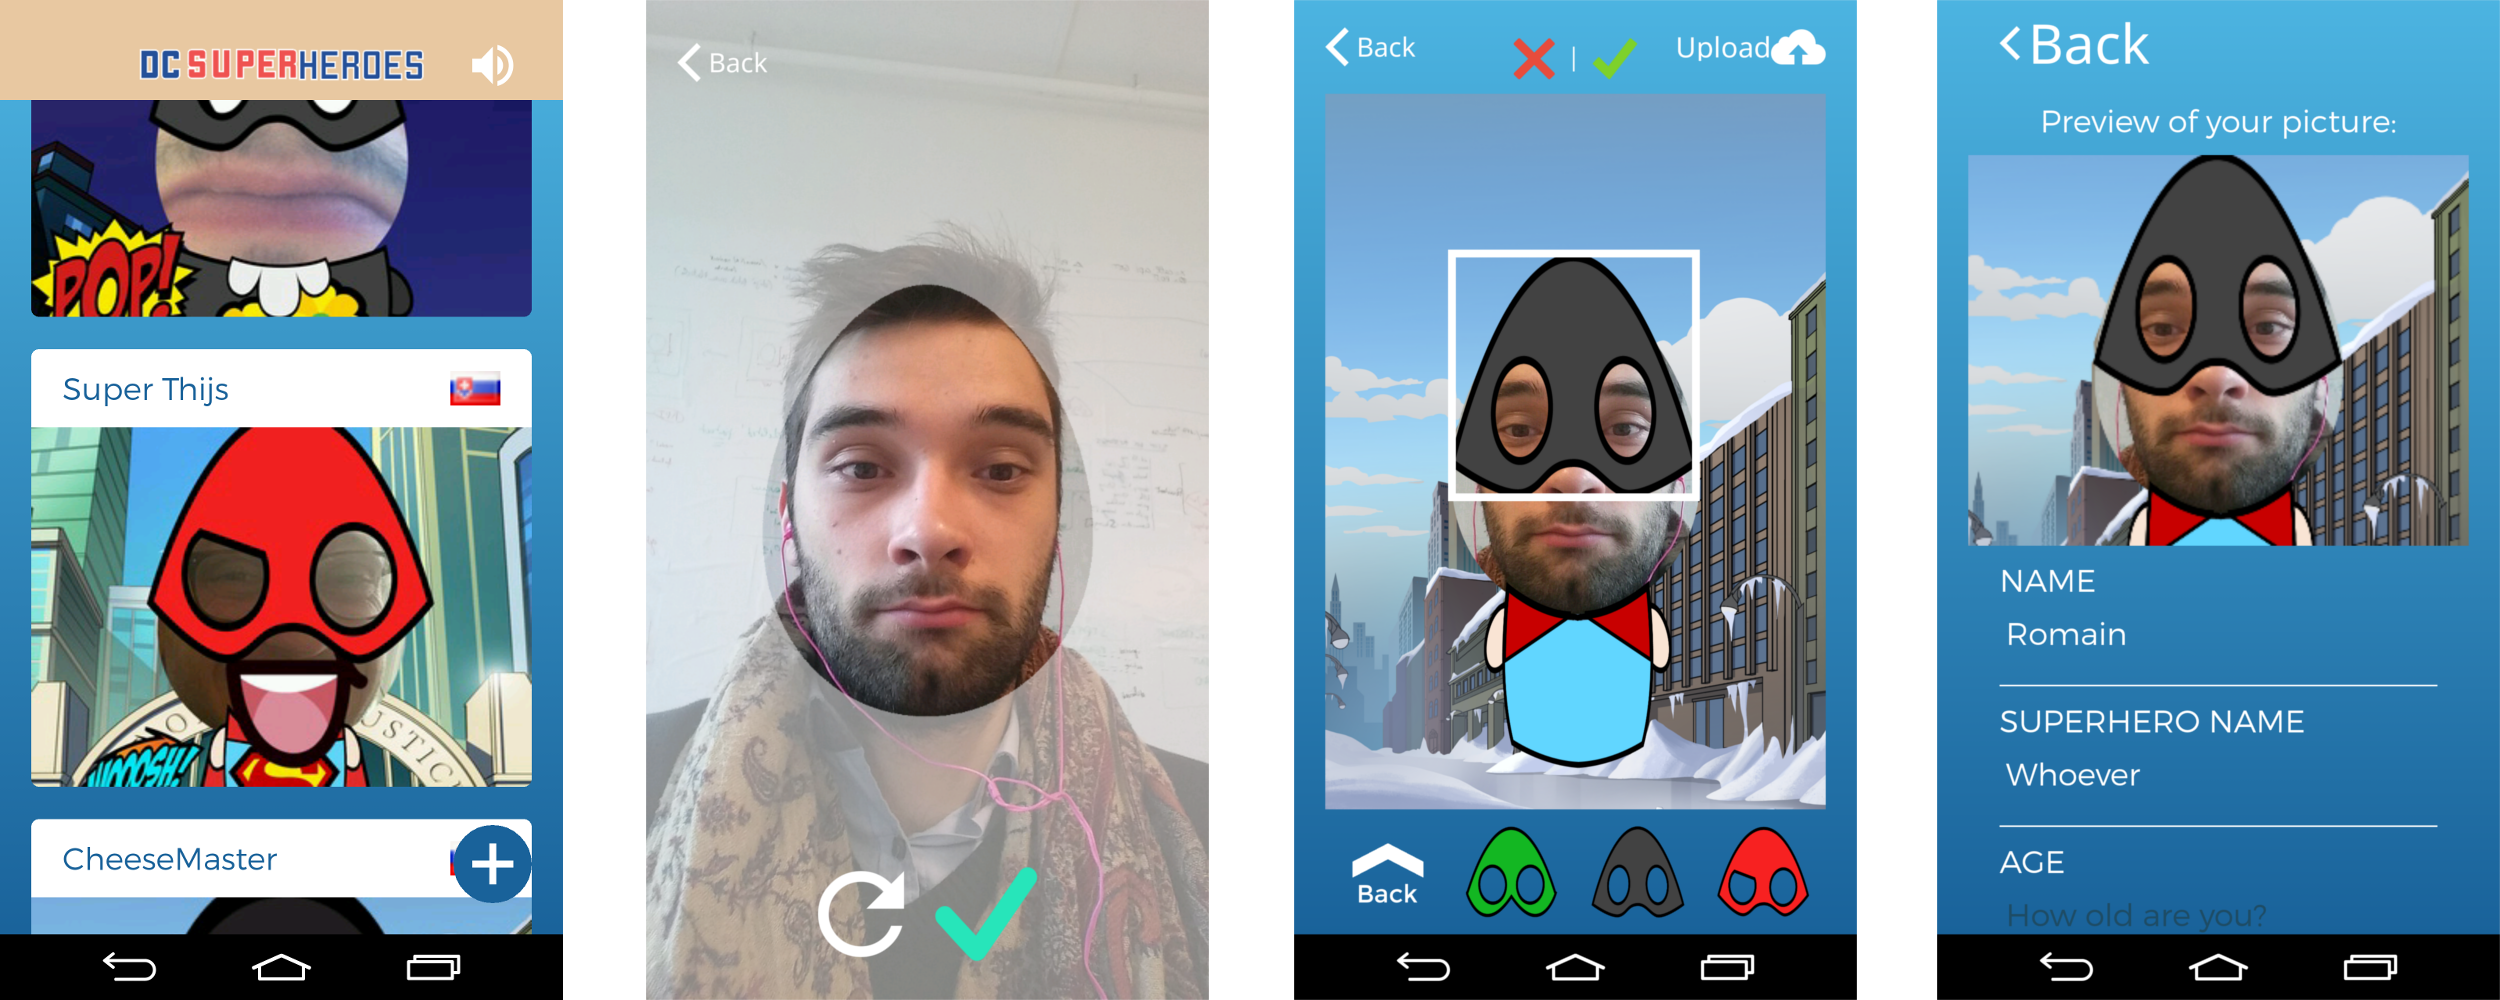
\includegraphics[width=1.00\textwidth]{images/tesco-screens.png}
   \caption[The different pages of the app DC Comics]{From left to right: Feed of pictures, Taking a selfie, Editing the selfie, Uploading it}
\end{figure}

From a technical point of view, the most challenging part was definitively being able to reproduce native capabilities with Titanium, here \textit{drag-and-drop} and \textit{pinch-to-zoom} (used while editing the selfie, third screenshot from left). Matthias took care of this. As for me, I was in charge of the selfie itself (second screenshot). I re-used a widget developed by Nguyen\footnote{\href{https://github.com/TheSmiths-Widgets/ts.camera}{github.com/TheSmiths-Widgets/ts.camera}} (our remote Vietnamese developer). Under the hood, his widget is using two Titanium modules (one for Android and another one for iOS), bringing camera support. His widget acts more as a bridge for our app, adding another layer of abstraction of top of the two modules. However, I had to tweak it a bit to fit at best our requirements. We needed it to be highly flexible regarding positioning and sizing, as the Android ecosystem includes tons of different screens. Pierre was responsible for the upload (last screenshot).

\medskip

After struggling a bit with layouts, I eventually came up with something working. I jumped onto another part of the project, the login page, which was pretty easy to develop. Two text inputs, a call to our REST API, and finally giving some feedback to the user. I forgot to mention, but with this project once again, we decided to go with \href{http://www.parse.com/}{www.parse.com}. We did not even develop our own API, we simply used the one provided natively by Parse to access and manipulate classes\footnote{\href{https://parse.com/docs/rest/guide}{parse.com/docs/rest/guide}}.

\subsection{Managing the screens flow}

Near the end of the project, after reviewing the app, I got assigned the screen flow. The way the end-user would go from one screen to another one, stacking the screens, closing them at the right time. The solution I decided to implement meets a logical flow, quite natural to users.

\begin{enumerate}
  \item From the feed, the users can start creating a new picture, by pressing a button. A new screen with the camera embedded appears.
  \item They can take a selfie and re-try as many times as they want (thanks to a button). When satisfied with the selfie, the editor is launched by pressing another button. The selfie screen is added to a stack of controllers to be closed.
  \item From the editor, users can go back to the selfie screen by pressing "Back" on top of the screen, or the Android-specific back button.
  \item When done with editing, the upload screen appears and the editor is added to the stack (which now contains two controllers).
  \item Here again, users can go back to the editor screen by pressing "Back" on top of the screen, or the Android-specific back button.
  \item The user now fills few input texts and uploads the picture. At the end of the upload, the user can either go back to the feed or take another picture. The current controller (upload) adds itself to the stack of controllers. Then it opens the selfie controller if needed. Eventually, it closes each controller from the stack, one by one (including itself).
  \item When the user goes back to the feed (if they chose to do so), the feed refreshes itself (thanks to an event triggered, '\lstinline{focus}', which fundamentally means that the controller just acquired the focus back).
\end{enumerate}

The following piece of code shows how a controller adds itself to the list of controllers to be closed.

\lstset{
    numbers=left
}
\javascript
\begin{lstlisting}
const args = arguments[0]; // arguments received from another controller at launch

...

// Launching another controller, here the editor starts the upload controller
Alloy.createController('upload', {
    picture: picture,
    toBeClosed: [$.container].concat(args && args.toBeClosed ? args.toBeClosed : [])
})
\end{lstlisting}
\lstset{
    numbers=none
}

The line 8 shows exactly how the controller adds itself (\lstinline{$.container}) to the already existing stack (array actually, the order does not matter) of controllers. As one can see, it also passes that stack to the next controller.\\
Below is how the final controller closes them all and redirects the user to either the feed or the selfie screen:

\begin{lstlisting}
if (e.goto == null || e.goto !== 'feed') {
    Alloy.createController('selfie');
}
[$.container].concat(args && args.toBeClosed ? args.toBeClosed : []).forEach(function(container) {
    if (container != null) {
        container.close();
    }
});
\end{lstlisting}
This controller management is pretty simple but yet works as expected.

\section{Conclusion}

We met the deadline. As I am writing theses lines (January, \nth{22}), we just finished the app. We are now waiting for accesses to the stores (Android and Apple), should we receive them anytime soon from our client.

\medskip

This project did put us under pressure, mostly because of the tight schedule. Manipulating graphical elements was very challenging as well. Every time Matthias would fix the editor, we would detect weird bugs, not to mention the huge differences between Android and iOS.

At last, we made it. We are pretty proud of the final product, and had a lot of fun developing it. I must admit that the app itself is really amusing and we hope the employees will enjoy it as much as we did.

\medskip

Regarding the technical aspects, we used the same tools as with our previous projects, nothing new. We faced big problems with Titanium, mainly due to a lack of consistency across platforms (Android and iOS). Sometimes, the app would not behave the same way, on different platforms, which convinced me cross-platform is not well suited for such specific projects. It rather fits simple projects that do not involve complex UI stuff. Camera management was kind of harsh as well.